\documentclass{article}
\usepackage[utf8]{inputenc}
\usepackage[italian]{babel}
\usepackage{amsmath}
\usepackage{amssymb}
\usepackage{siunitx}
\usepackage{tabularray}
\usepackage{graphicx}
\usepackage{float}
\usepackage{minted}
\usepackage[page]{appendix}
\usepackage{mathtools}
\newcommand*{\diam}{\varnothing}
\newcommand*{\acqua}{{\text{H}_2\text{O}}}
\newcommand*{\best}[1]{{#1}_\text{best}}
\newcommand*{\bestp}[1]{{\left(#1\right)}_\text{best}}
\newcommand*{\pbest}[1]{\left({#1}_\text{best}\right)}
\newcommand*{\pbestp}[1]{\left({\left(#1\right)}_\text{best}\right)}
\newcommand*{\errrel}[1]{\frac{\delta #1}{{#1}_\text{best}}}
\title{
    Laboratorio di Fisica 1\\
    R6: Calorimetro delle mescolanze
}
\author{Gruppo 17: Bergamaschi Riccardo, Graiani Elia, Moglia Simone}
\date{6/12/2023 – 13/12/2023}
\makeindex
\begin{document}

\maketitle

\begin{abstract}
    Il gruppo di lavoro ha misurato il calore specifico di tre solidi distinti
    per risalirne alla natura; a questo fine, è stato necessario determinare
    le caratteristiche termiche del calorimetro
    (capacità termica, tempo caratteristico e conducibilità).
\end{abstract}

\setcounter{section}{-1}
\section{Materiali e strumenti di misura utilizzati}
\begin{center}
    \begin{tblr}{ |Q[l,m]|Q[c,m]|Q[c,m]|Q[c,m]| }
        \hline
        \textbf{Strumento di misura} & \textbf{\:\:\:\:\:Soglia\:\:\:\:\:} & \textbf{Portata} & \textbf{Sensibilità} \\
        \hline
        Termometro digitale & $\qty{0.1}{\degree C}$ & N./A. & $\qty{0.1}{\degree C}$ \\
        \hline[dashed]
        Cronometro & $\qty{0.5}{s}$ & N./A. & $\qty{0.5}{s}$ \\
        % \hline[dashed]
        % Termometro a mercurio & $\qty{0.1}{\degree C}?$ & $\qty{100}{\degree C}?$ & $\qty{0.1}{\degree C}?$ \\
        \hline[dashed]
        Barometro & N./A. & $\qty{14000}{hPa}$ & $\qty{1}{hPa}$ \\
        \hline[dashed]
        Cilindro graduato & $\qty{1}{mL}$ & $\qty{100}{mL}$ & $\qty{1}{mL}$ \\
        \hline[dashed]
        Bilancia di precisione & $\qty{0.01}{g}$ & $\qty{4100.00}{g}$ & $\qty{0.01}{g}$ \\
        \hline
        \textbf{Altro} & \SetCell[c=3]{l} \textbf{Descrizione/Note} \\
        \hline
        \hline
        Calorimetro & \SetCell[c=3]{l} {Quasi adiabatico.} \\
        \hline[dashed]
        {Fornelletto e pentolino} & \SetCell[c=3]{l} {Per scaldare acqua e campioni.} \\
        \hline[dashed]
        Tre campioni solidi & \SetCell[c=3]{l} {Li chiameremo $A$, $B$ e $C$.} \\
        \hline
    \end{tblr}
\end{center}

\section{Misurazione della massa equivalente}

Il calorimetro, per quanto isolante termicamente, comunque non è completamente
adiabatico. Pertanto, prima di procedere con la misura indiretta dei calori
specifici dei campioni di materiale ignoto, è necessario ottenere una stima
della capacità termica del calorimetro $C_\text{cal}$.

Per semplificare i calcoli, abbiamo definito “massa (d'acqua) equivalente
(in senso termico) al calorimetro” come la quantità:
\[m_\text{eq} \coloneqq \frac{C_\text{cal}}{c_{\text{H}_2\text{O}}}\]

\emph{
\textbf{Osservazione.} La massa equivalente ci dà anche un'idea di
quanto il calorimetro disturbi le misure.
}

\subsection{Esperienza e procedimento di misura}

\emph{
\textbf{Nota.} La temperatura di ebollizione ($T_\text{db}$) dell'acqua distillata
dipende dalla pressione atmosferica. Per questo motivo, abbiamo misurato la pressione
atmosferica, ottenendo un valore di $\left(992\pm1\right)\unit{hPa}$, al quale, secondo la
letteratura, corrisponde un punto di ebollizione dell'acqua di $\left(99.4\pm0.1\right)\unit{\degree C}$.
}

\begin{enumerate}
    \item
        Misuriamo, mediante la bilancia di precisione, la massa del
        calorimetro vuoto (coperchio compreso):
        $m_\text{cal} = \left(781.91\pm0.01\right) \unit{g}$
    \item
        Versiamo, aiutandoci col cilindro graduato, circa $\qty{100}{mL}$
        di acqua distillata ($c_{\text{H}_2\text{O}}=\qty{4186}{J\,kg^{-1}K^{-1}}$)
        a temperatura ambiente $T_\text{amb}$ nel calorimetro.
        Per avere una stima più accurata di questa quantità di acqua,
        misuriamo la massa complessiva del calorimetro dopo questa operazione.
        In questo modo, otteniamo indirettamente la massa d'acqua “fredda”:
        $m_\text{fredda} = \left(99.35\pm0.02\right) \unit{g}$
    \item
        Scaldiamo nel pentolino altri $\qty{100}{mL}$, circa, di acqua distillata,
        fino al punto di ebollizione.
    \item
        Inserito nel calorimetro il termometro digitale, avviamo l'acquisizione dati
        (a intervalli di $\qty{0.5}{s}$).
        Riapriamo poi il calorimetro e vi versiamo all'interno,
        velocemente, l'acqua calda.
    \item
        Chiuso il calorimetro, mescoliamo lentamente l'acqua per assicurarci
        una distribuzione omogenea del calore, senza però introdurre una quantità
        significativa di energia all'interno del sistema.
    \item
        Dopo una decina di minuti, interrompiamo l'acquisizione, estraiamo il
        termometro e misuriamo nuovamente la massa del sistema.
        In questo modo, per differenza, otteniamo la massa dell'acqua calda che
        avevamo versato nel calorimetro\footnote{
        Si noti che questa massa è minore di quella che avevamo versato
        nel pentolino, poiché una parte dell'acqua è evaporata. Misurare la massa
        alla fine dell'esperimento, per differenza, ci permette di non doverne
        tener conto successivamente. Possiamo infatti considerare il calorimetro
        come un sistema chiuso: finché non lo apriamo, la massa complessiva
        non cambia.
        }:
        $m_\text{calda} = \left(85.12\pm0.03\right) \unit{g}$
\end{enumerate}

\emph{
\textbf{Osservazione.} È meglio che i due volumi d'acqua siano molto simili e che
la loro somma sia pressoché pari al volume che utilizzeremo nella seconda parte
dell'esperimento, in modo che il calorimetro si bagni allo stesso modo.
}

\subsection{Analisi dei dati raccolti e conclusioni}
Detta $T_\text{eq}$ la temperatura di equilibrio del sistema, vale:
\[
m_\text{calda} (T_\text{eb} - T_\text{eq}) =
(m_\text{fredda} + m_\text{eq})(T_\text{eq} - T_\text{amb})
\]
da cui:
\[
m_\text{eq} = \frac{T_\text{eb}-T_\text{eq}}{T_\text{eq}-T_\text{amb}} m_\text{calda} - m_\text{fredda}
\]

Di seguito riportiamo, in un grafico, i dati raccolti dal termometro digitale.

\begin{center}
    \begin{figure}[H]
        % trim={< v > ^}
        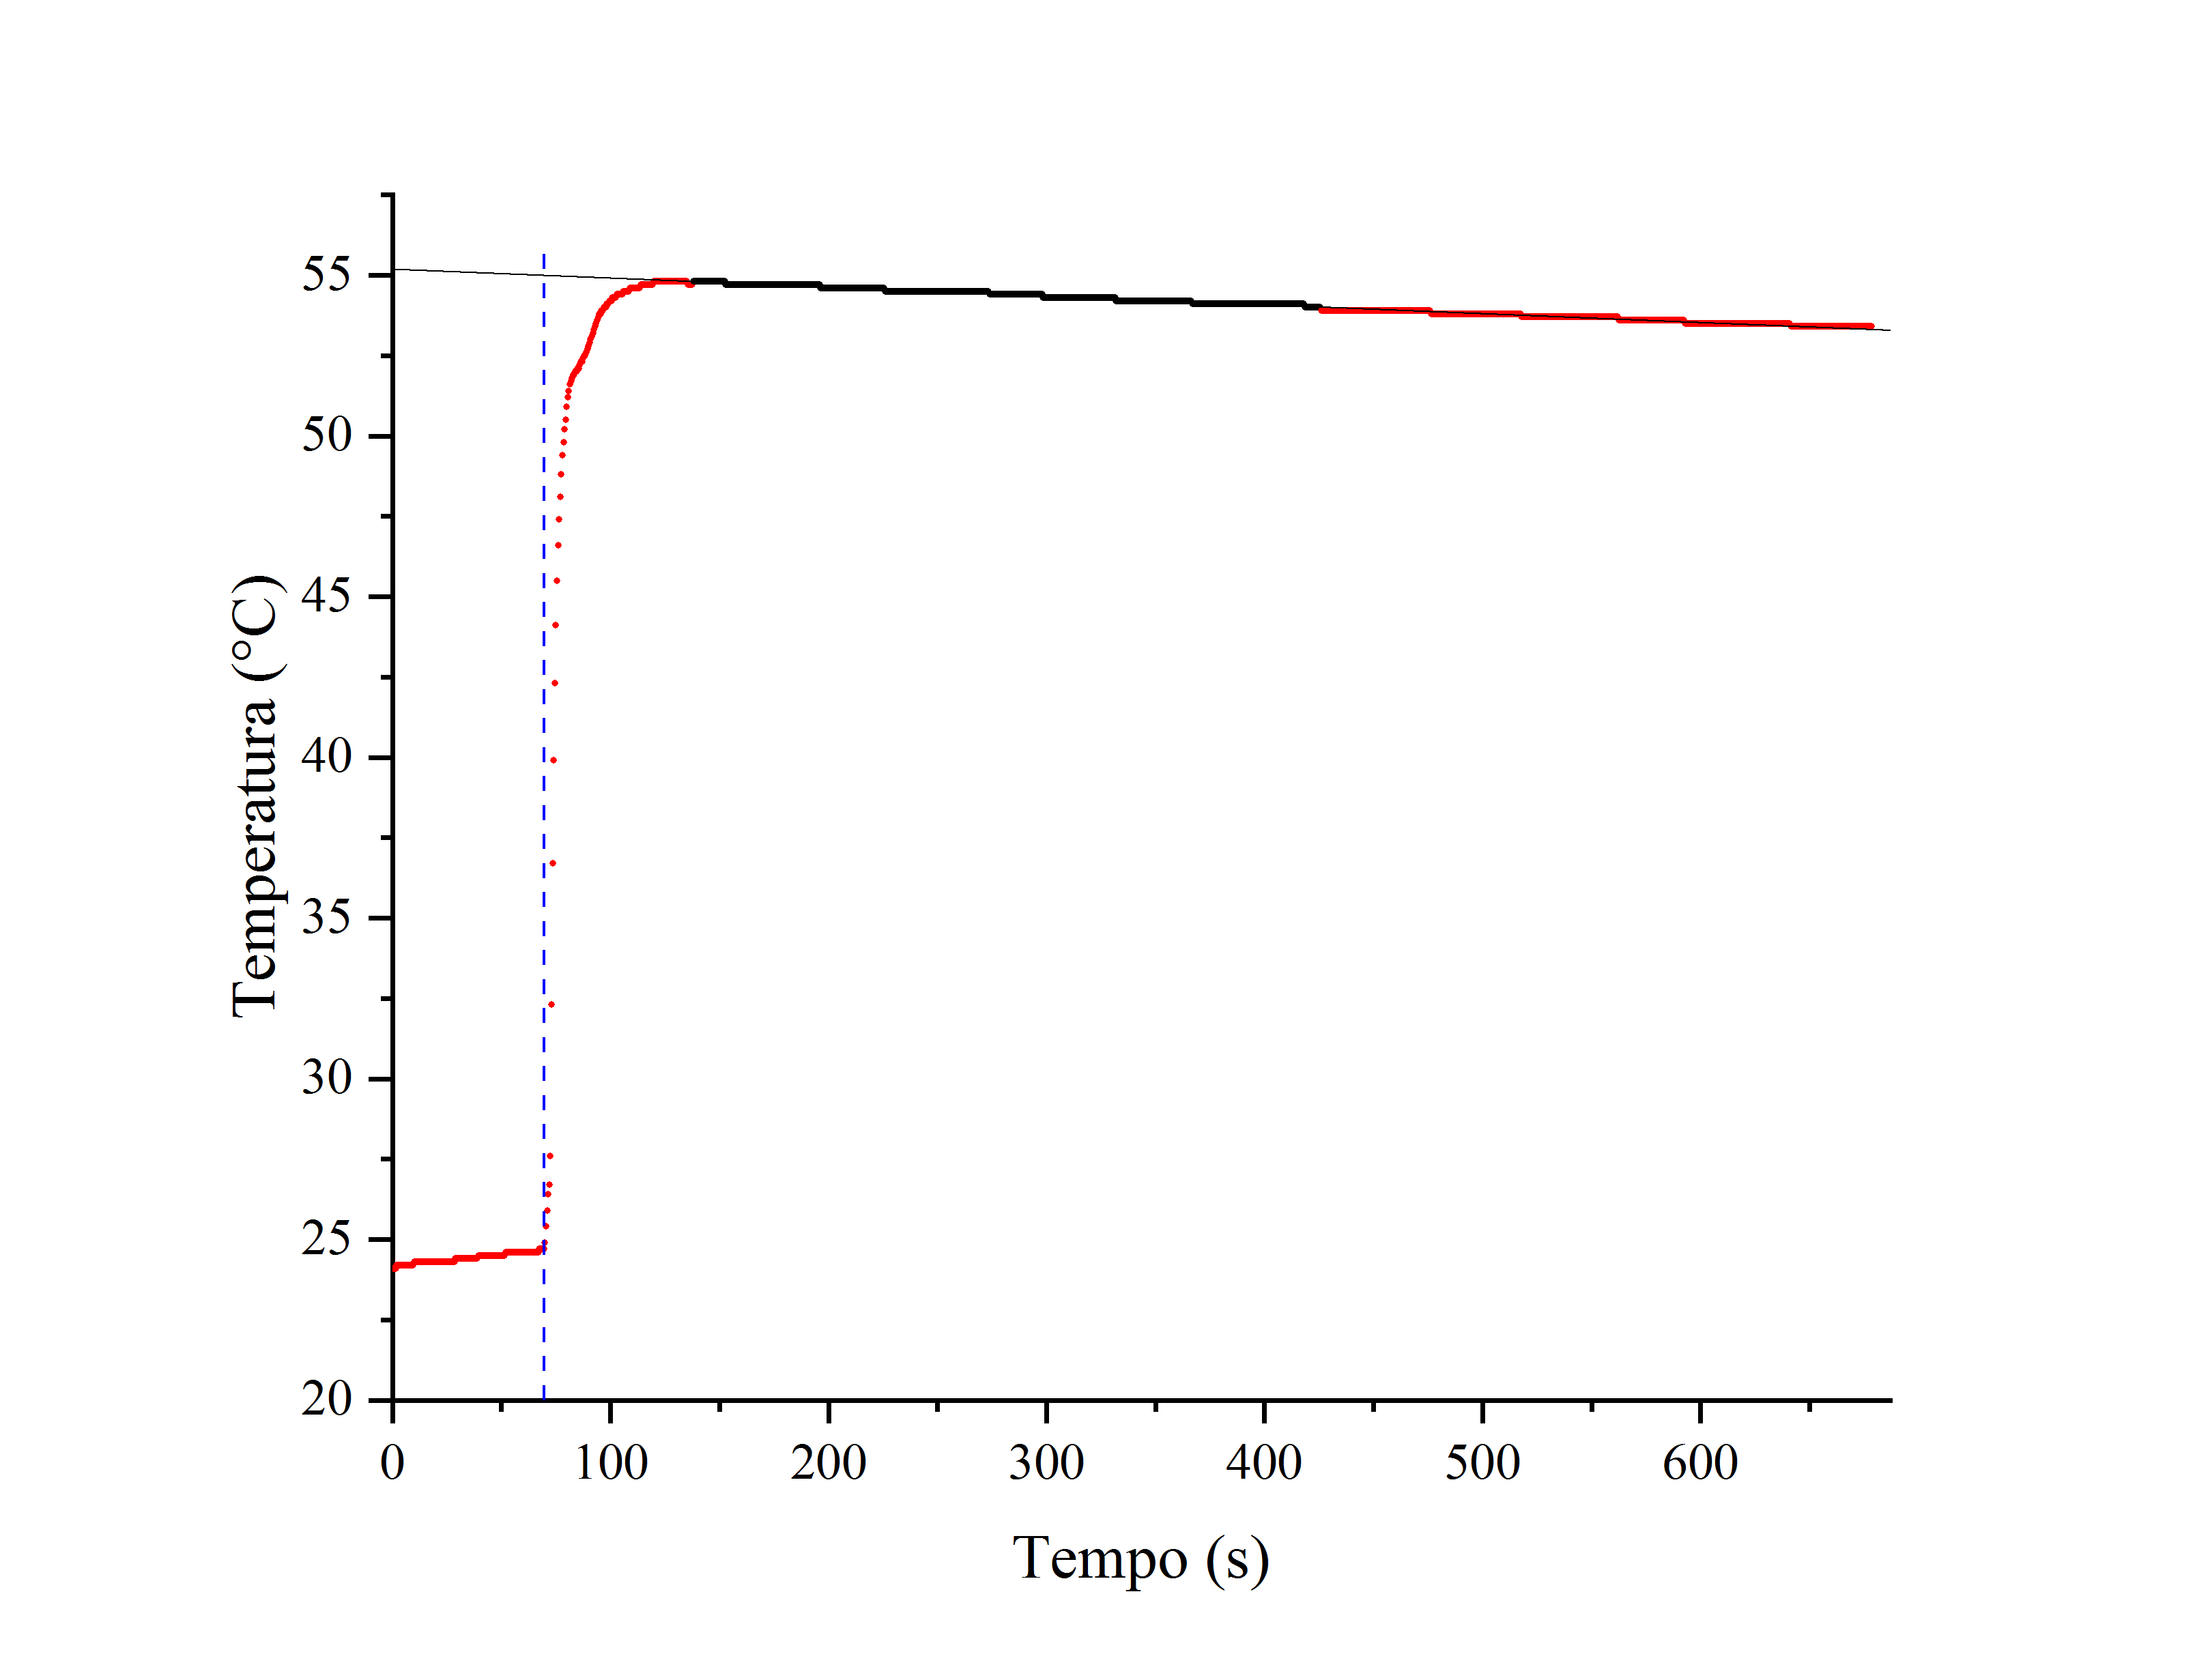
\includegraphics[trim={2cm 1cm 2cm 2.1cm},clip,width=\textwidth]{img/RegH2O.jpg}
        \caption{\emph{I dati raccolti col termometro.
        In nero, appena visibile, una retta di regressione sull'intervallo di dati indicato in nero.
        In blu, l'istante di tempo nel quale abbiamo inserito l'acqua calda.
        L'ordinata del punto di intersezione fra le due rette è la temperatura di equilibrio.
        }}
    \end{figure}
\end{center}

Abbiamo ottenuto $T_\text{eq} = \left(55.0\pm0.1\right)\unit{\degree C}$.
Utilizzando le relazioni sopra esposte, abbiamo calcolato\footnote{
    Avendo stimato gli errori come piccoli, casuali e indipendenti,
    abbiamo utilizzato la propagazione degli errori per calcolare tutte le
    incertezze delle misure indirette.
} $m_\text{eq} = \left(25\pm3\right)\unit{g}$.

Possiamo ora proseguire con la stima dei calori specifici dei vari campioni
metallici.

\pagebreak
\section{Misurazione del calore specifico dei campioni}

\subsection{Esperienza e procedimento di misura}

Per ogni campione $i\in\left\{A,B,C\right\}$:

\begin{enumerate}
    \item
        Versiamo nel pentolino una quantità d'acqua tale da permettere l'immersione
        completa del campione in essa e la portiamo ad ebollizione.
    \item
        Con l'aiuto del calibro ventesimale e di una cordicella, sospendiamo il
        campione all'interno dell'acqua, nel pentolino, in modo tale che non tocchi
        il fondo e, contemporaneamente, sia immerso completamente.
    \item
        Versiamo circa $\qty{200}{mL}$ di acqua distillata, a temperatura ambiente
        ($T_\text{amb}$), nel calorimetro (vuoto e asciutto).
        Ne misuriamo la massa $m_\acqua$ per differenza, secondo quanto descritto
        al paragrafo 1.1.
    \item
        Misuriamo la massa $m_i$ del campione con la bilancia di precisione.
    \item
        Quando il campione raggiunge la stessa temperatura dell'acqua ($T_\text{eb}$),
        inseriamo il termometro nel calorimetro e avviamo l'acquisizione dati.
        Poi, apriamo velocemente il calorimetro per inserirvi inseriamo il campione.
    \item
        Chiuso il calorimetro, mescoliamo lentamente l'acqua per assicurarci
        una distribuzione omogenea del calore, senza però introdurre una quantità
        significativa di energia all'interno del sistema.
    \item
        Dopo una decina di minuti, interrompiamo l'acquisizione.
\end{enumerate}

\subsection{Analisi dei dati raccolti e conclusioni}
Detta $T_\text{eq}$ la temperatura di equilibrio, per ogni campione
$i\in\left\{A,B,C\right\}$ vale:
\[
    c_i m_i (T_\text{eb} - T_\text{eq}) =
    c_\acqua (m_\acqua + m_\text{eq}) (T_\text{eq} - T_\text{amb})
\]
dove $c_i$ è il calore specifico del campione. Risolvendo in $c_i$ otteniamo:
\[
    c_i = c_\acqua\cdot\frac{m_\acqua + m_\text{eq}}{m_i}
          \cdot\frac{T_\text{eq} - T_\text{amb}}{T_\text{eb} - T_\text{eq}}
\]

Nella seguente tabella riportiamo quanto calcolato a partire dai dati raccolti.
In tutti i casi, $T_\text{eq}$ è stata calcolata secondo quanto descritto al
paragrafo 1.2.

\begin{center}
\begin{tabular}{ |c|c|c|c|c|c| }
    \hline
    $i$ & $m_\acqua$ ($\unit{g}$) & $m_i$ ($\unit{g}$) & $T_\text{amb}$ ($\unit{\degree C}$) & $T_\text{eq}$ ($\unit{\degree C}$) & $c_i$ ($\unit{J\,{kg}^{-1}{K}^{-1}}$) \\
    \hline
    $A$&$197.54\pm0.02$&$12.43\pm0.01$&$24.7\pm0.1$&$25.2\pm0.1$ & $500\pm200$ \\
    $B$&$194.81\pm0.02$&$28.73\pm0.01$&$25.1\pm0.1$&$25.9\pm0.1$ & $350\pm100$ \\
    $C$&$194.00\pm0.02$&$44.86\pm0.01$&$25.6\pm0.1$&$26.0\pm0.1$ & $110\pm60$ \\
    \hline
\end{tabular}
\end{center}

Per capire di che materiale siano composti i campioni abbiamo confrontato i valori
di $c_i$ calcolati con le misure indicate in letteratura ($c_\text{met}$).

Per valutare numericamente la consistenza dei risultati ottenuti con i valori attesi,
abbiamo calcolato, per ogni combinazione campione-materiale, il seguente valore (numero puro):
\[\varepsilon = \frac{c_i - c_\text{met}}{\delta c_i + \delta c_\text{met}}\]
Allora $c_i$ è consistente con $c_\text{met}$ se e solo se $\left|\varepsilon\right|\le 1$.

\begin{center}
\begin{tblr}{ |c|c|c|c|c| }
    \hline
    $i$ & $c_i$ ($\unit{J\,kg^{-1}K^{-1}}$) & Metallo $m$ & $c_m$ ($\unit{J\,kg^{-1}K^{-1}}$) & $\varepsilon$ \\
    \hline
    $A$ & $500\pm200$ & Acciaio inox & $502 \pm 1$ & $+0.018$ \\
    \hline[dashed]
        &             & Ottone  & $377 \pm 1$ & $-0.279$ \\
    $B$ & $350\pm100$ & Rame    & $385 \pm 1$ & $-0.359$ \\
        &             & Zinco   & $388 \pm 1$ & $-0.389$ \\
    \hline[dashed]
    $C$ & $110\pm60$  & Piombo  & $130 \pm 1$ & $-0.305$ \\
    \hline
\end{tblr}
\end{center}

\emph{
    \textbf{Osservazione.}
    È interessante notare come ottone, rame e zinco abbiano calori specifici piuttosto vicini
    fra loro e siano tutti compatibili con le nostre misure: in effetti, l'ottone è proprio
    una lega di rame e zinco. Riteniamo che il nostro campione sia di ottone, principalmente
    a causa della sua colorazione.
}

\section{Misurazione del tempo caratteristico del calorimetro}

\subsection{Esperienza e procedimento di misura}

\begin{enumerate}
    \item
        Scaldiamo, nel pentolino, circa $\qty{200}{mL}$ di acqua distillata
        fino al punto di ebollizione.
    \item
        Inseriamo il termometro nel calorimetro, vuoto e asciutto, e avviamo
        l'acquisizione dati.
    \item
        Aperto il calorimetro, vi versaimo l'acqua, per poi richiuderlo velocemente.
        Acquisiamo dati per un tempo complessivo di $\qty{2845}{s}$, ovvero
        $\qty{47}{min}\qty{25}{s}$.
    \item
        Al termine dell'acquisizione, prima di riaprire il calorimetro, estraiamo
        il termometro e misuriamo nuovamente la massa complessiva, sempre per
        determinare la quantità d'acqua calda inizialmente introdotta.
\end{enumerate}

\subsection{Analisi dei dati raccolti e conclusioni}
Su larga scala, l'andamento della temperatura all'interno del calorimetro
in funzione del tempo è esponenziale. In particolare, $T(t)$ segue questa
legge:
\[
    T(t) = (T_0 - T_\text{amb}) e^{-t/\tau} + T_\text{amb}
\]
dove $\tau$ è il cosiddetto “tempo caratteristico”, un parametro legato
alla conducibilità termica: vale infatti
\[\kappa = \frac{C_\text{cal}}{\tau} = \frac{c_\acqua m_\text{eq}}{\tau}\].

Riarrangiando l'equazione precedente, si ottiene\footnote{
    A patto, ovviamente, che $T(t) > 0 \forall t$.
    Nel caso dei nostri dati, cio è vero in particolare
    a partire dal momento in cui $T(t)$ assume l'andamento
    esponenziale.
}:
\[
    \ln(T(t) - T_\text{amb}) = -1/\tau t + \ln(T_0 - T_\text{amb})
\]
È pertanto possibile determinare $\tau$ mediante una regressione lineare (pesata\footnote{
    A causa della trasformazione applicata ai dati ($T \longmapsto \ln(T - T_\text{amb})$),
    gli errori assoluti su $\ln(T(t) - T_\text{amb})$ variano notevolmente. Per leggibilità,
    \emph{non} abbiamo riportato le barre di errore nei grafici; tuttavia, abbiamo
    considerato le incertezze in ogni calcolo, utilizzando, ove necessario, la propagazione
    degli errori, come sottolineato alla nota 2.
}):

\begin{center}
    \begin{figure}[H]
        % trim={< v > ^}
        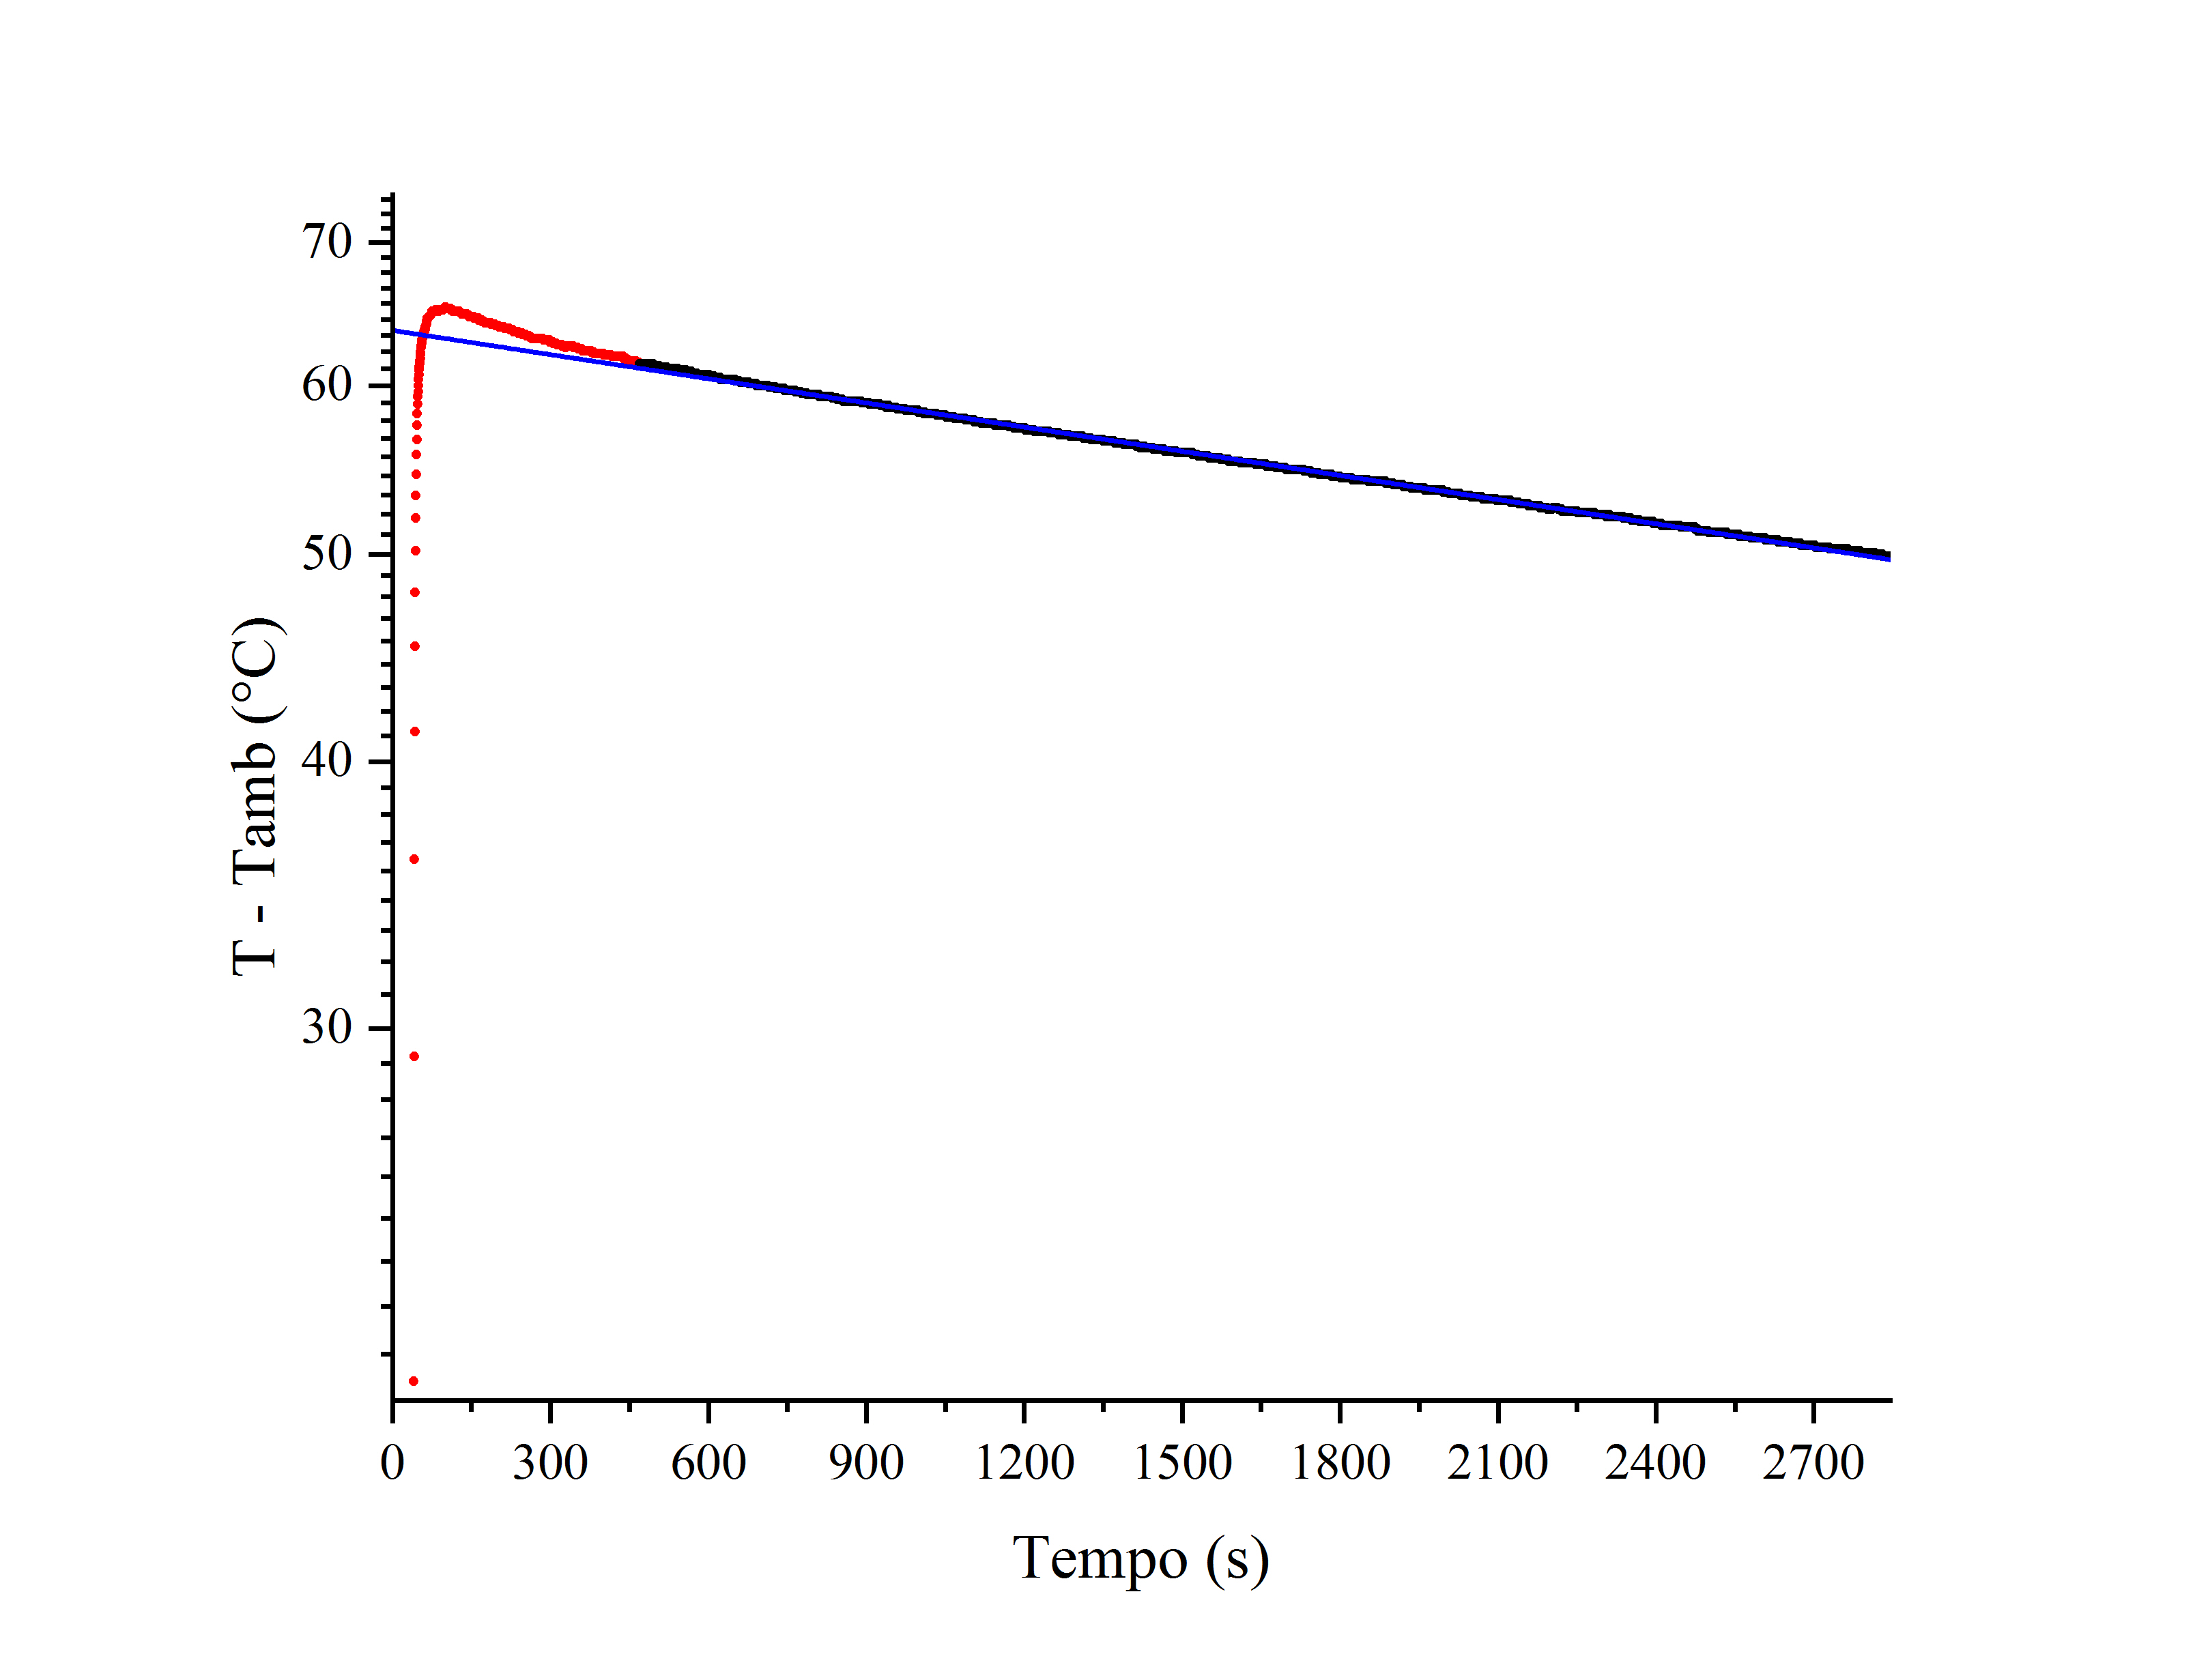
\includegraphics[trim={2cm 1cm 2cm 2.1cm},clip,width=\textwidth]{img/LogLinFit.jpg}
        \caption{\emph{I dati che abbiamo utilizzato per la regressione lineare.
        In blu, la retta di regressione sull'intervallo di dati indicato in nero.
        }}
    \end{figure}
\end{center}
\begin{center}
    \begin{figure}[H]
        % trim={< v > ^}
        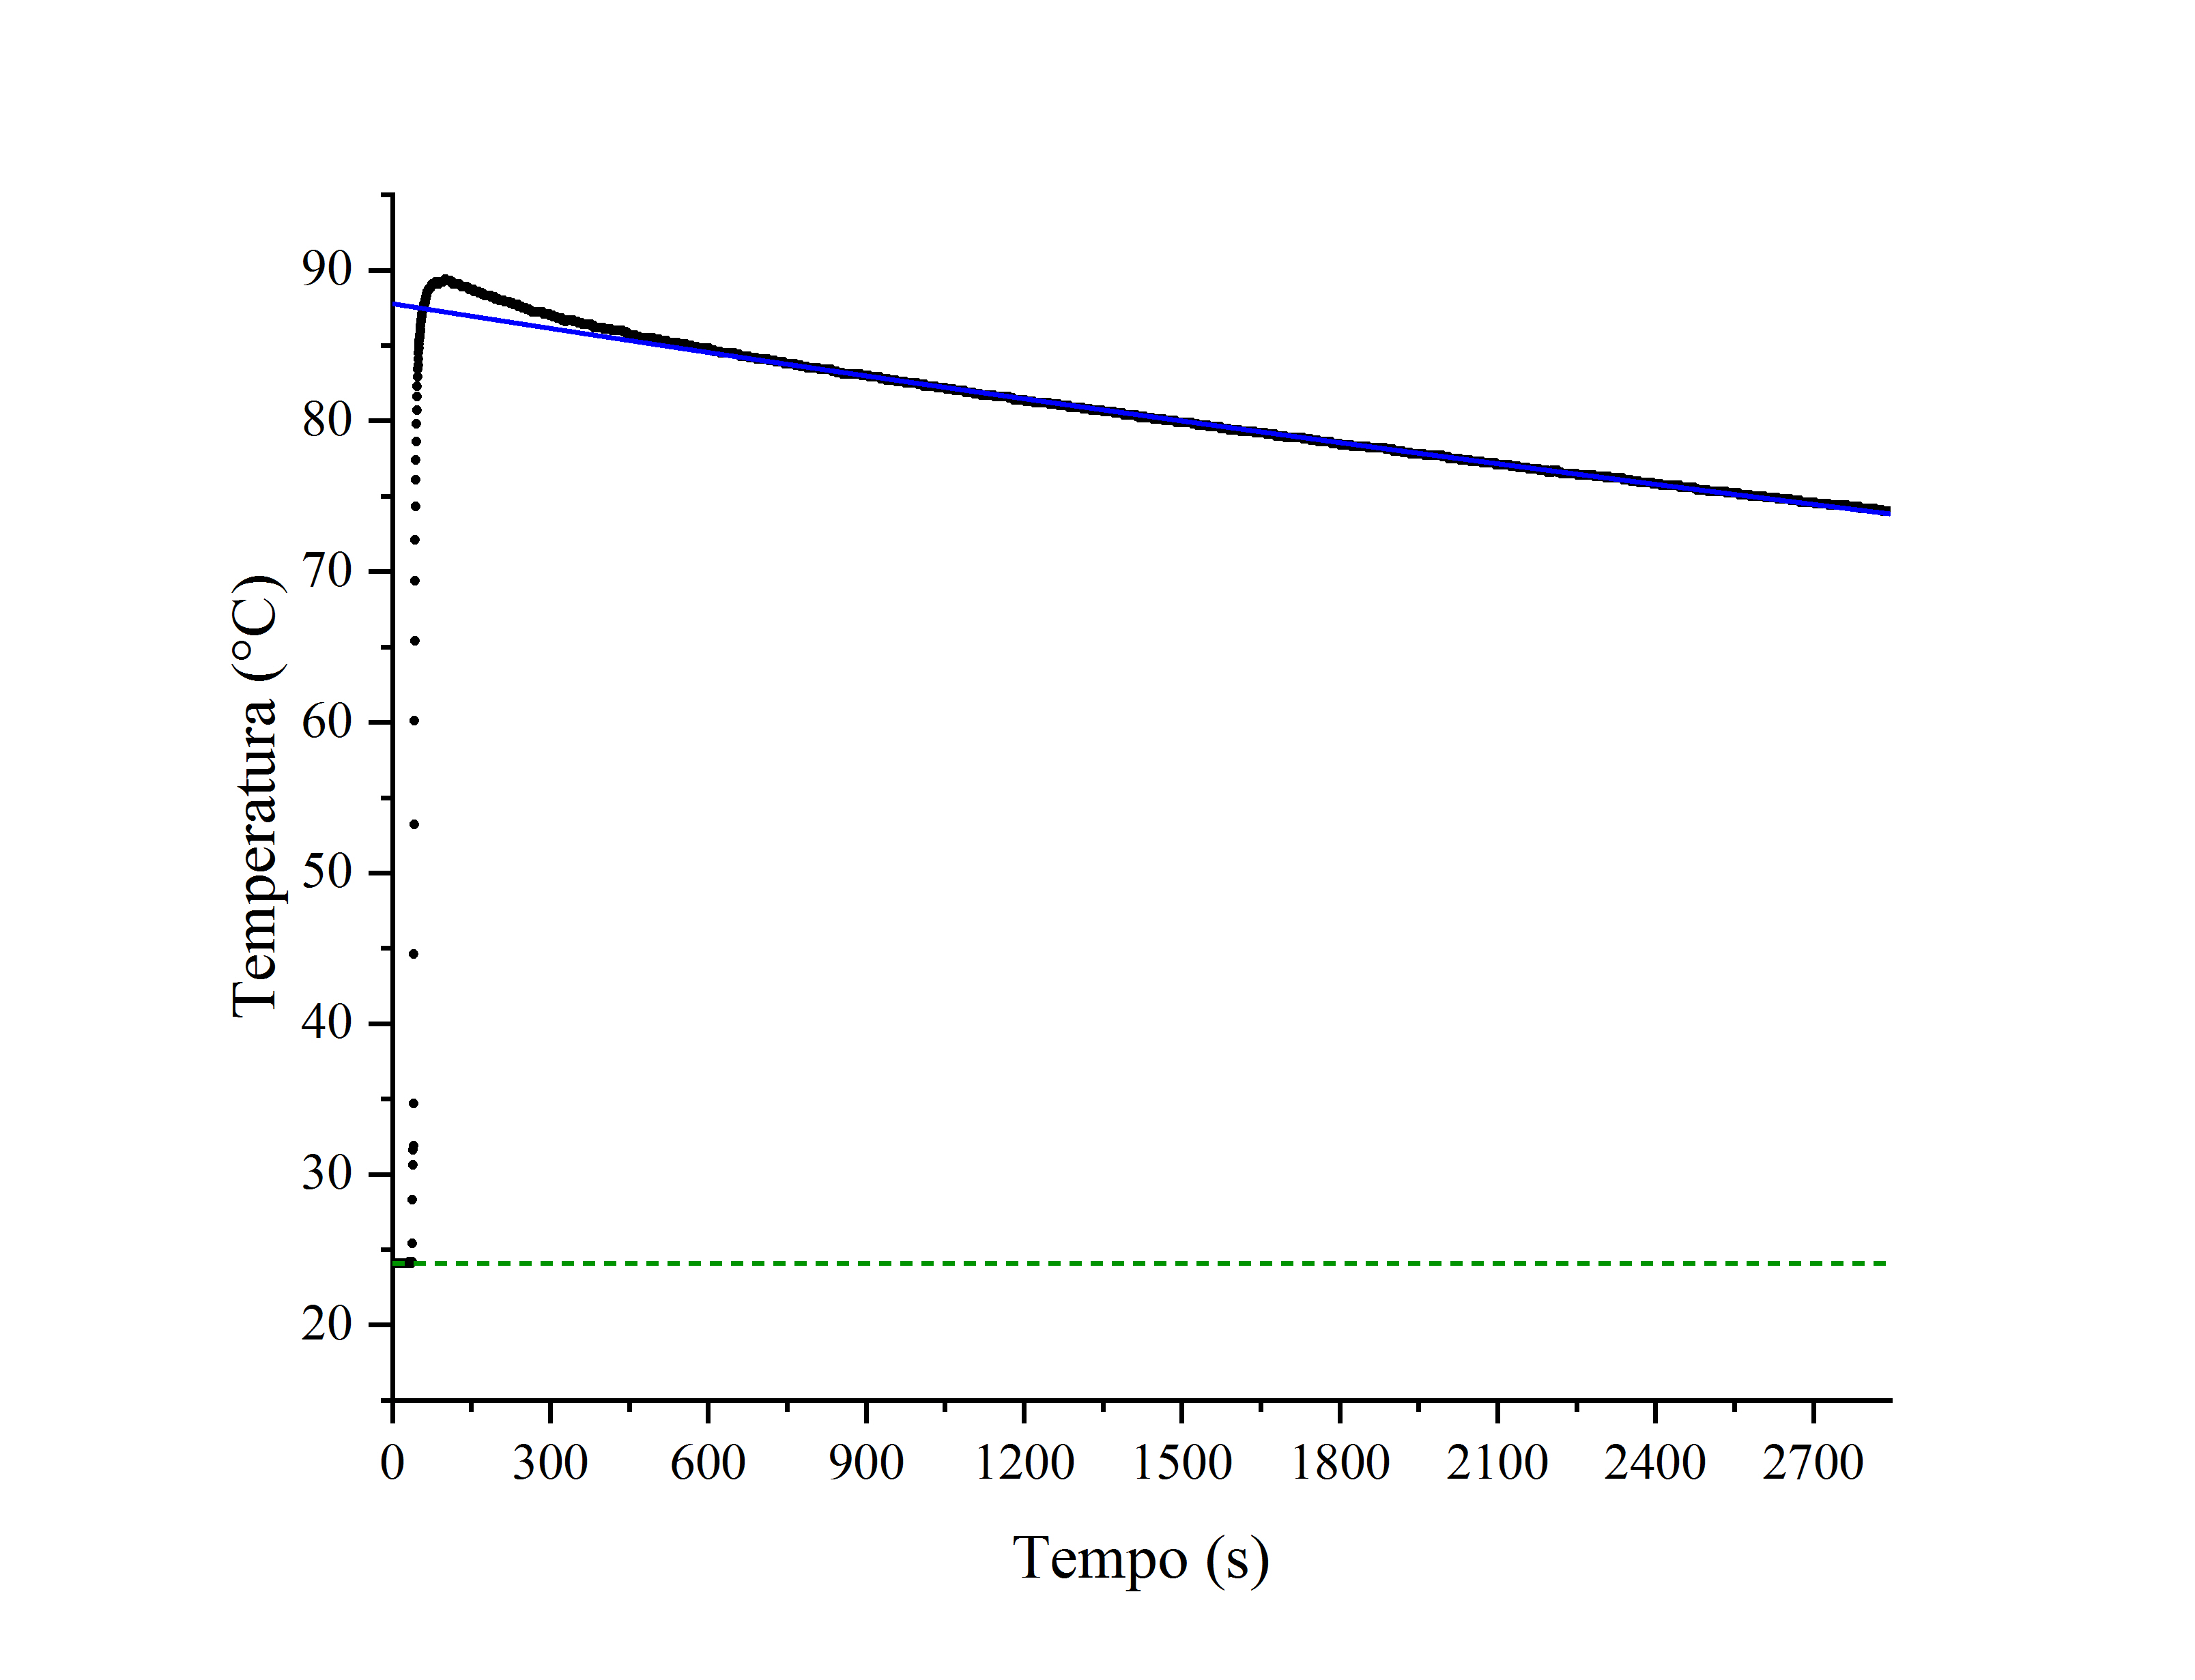
\includegraphics[trim={2cm 1cm 2cm 2.1cm},clip,width=\textwidth]{img/ExpFit.jpg}
        \caption[]{\emph{I dati raccolti col termometro.
        In blu, la curva esponenziale così ottenuta.
        In verde, la temperatura ambiente.
        }}
    \end{figure}
\end{center}

Dalla regressione lineare emerge che $\tau = \left(11.510\pm0.014\right)\unit{ks} = \qty{191}{min}\qty{50}{s}\pm\qty{14}{s}$.
Pertanto $\kappa = \left(9.3\pm1.1\right)\unit{W\,K^{-1}}$.

\end{document}
